%This work was supported by the Institute of Systems Engineering, Macau University of Science and Technology.
%!TEX program 	= xelatex
\PassOptionsToPackage{quiet}{xeCJK}
\documentclass{format/MUSTThesisC}

% redeclare 
\newfontscript{CJK}{hani} 
% \newfontscript{CJK~Ideographic}{hani} 
\ExplSyntaxOff  
\usepackage{xeCJK}



\usepackage{amsmath,amssymb, amsfonts,amsthm}


\renewcommand{\figurename}{{Fig.}}
\renewcommand{\tablename}{{Table}}

%%%%%%%%%%%%%%%%%%%%%
%
% Here one can add any package whenever necessary
%
%%%%%%%%%%%%%%%%%%%%%%


\usetikzlibrary{arrows.meta,arrows,shapes,automata,backgrounds,petri,patterns,decorations.pathmorphing,positioning,calc,shapes.geometric}%插件
\usepackage{xcolor}
\usepackage{tcolorbox}
\usepackage{algorithmic}
\usepackage{diagbox}
\usepackage[ruled,vlined,linesnumbered]{algorithm2e}
\usepackage{tabu}

\usepackage{hyperref}
\hypersetup{
    colorlinks=true,
    linkcolor=black,
    filecolor=magenta,      
    urlcolor=blue,
    pdftitle={Overleaf Example},
    pdfpagemode=FullScreen,
    }

%\usepackage{xeCJK}

\begin{document}





% -------------------------------------------------<< 增加 MUST 校徽水印-----論文終稿使用

\AddToShipoutPicture{\BackgroundPic}

% The watermark line can be commented out when editing. After the thesis is done, one can recover this line such that the watermark is exposed (若水印影响编辑可先注释掉,完成后在加水印).

%% -------------------------------------------------<< 自動生成 MUST 指定格式的扉頁
\def\Ctitle 		{論文標題}
\def\Etitle 		{Thesis title}
\def\Sname 			{王茗琛}
\def\Sno 			{2230025907}
\def\Sfaculty 		{創新工程學院}
\def\Sprogram 		{智能技術碩士}
\def\Smajor 		{智能技術碩士}
\def\Ssupervisor	{劉新}
\def\Sdate			{YYYY/MM/DD}

% 自動生成論文扉頁
\mustTitle



%% -------------------------------------------------<< \mustCabstract 生成中文摘要
\mustCabstract
{
	% 引用目錄下的文件內容
	離線手寫簽名驗證是生物特徵技術的一個應用场景, 其根據用戶提供的手寫簽名与資料庫中該用戶存儲的手寫簽名進行對比以驗證用戶身份, 在日常生活中被廣泛用於安全認證, 金融交易等安全領域. 學術研究中, 離線手寫簽名驗證定義為作者獨立和作者依賴任務. 第一種任務是將手寫簽名與對應作者的參考簽名進行對比驗證. 第二種任務是在作者依賴任務的基礎上使用獨立的作者分類器判斷輸入簽名是否是偽造的.

本工作内容如下: 1. 提出圖像多尺度融合特徵的OSVTF端到端模型結構,初步驗證模型架構性能. 2. 針對多尺度特徵融合和模型優化部分, 進行消融實驗以證實模型子網絡組合方案的性能. 3. 針對作者依賴任務,將對比支持向量機或全局平均池化作爲分類器的OSVTF性能.

在實驗部分, OSVTF模型在BHSig-B 80/20數據集的作者獨立和作者依賴任務中EER為4.54\%和2.13\%, 在BHSig-H 100/60數據集的EER為3.90\%和2.68\%. 在消融實驗部分, OSVTF在CEDAR 50/5數據集的作者獨立任務中EER為4.75\%. 結果證實采取了多尺度融合特徵的OSVTF能夠加强對僞造簽名的敏感部分特徵學習, 部分優化將加快模型訓練過程的收斂速度.


% 本文研究離散事件繫統的監督控制問題。
% 在使用該範本中有任何問題請聯繫覃濤
% \href{mailto:zhwli@ieee.org}{zhwli@ieee.org}。
% 澳門科技大學系統工程研究所感謝覃濤對設計此範本的貢獻。


% \medskip\medskip

% The template can be used in online and offline ways. For the former (highly recommended), 
% Overleaf (\url{https://www.overleaf.com}) is a collaborative cloud-based LaTeX editor used for writing, editing and publishing scientific documents, which is much easy to use and friendly. In overleaf, the compiling command is \textcolor{blue}{XeLatex}.

% For the latter, one can use Texstudio, which is a very popular yet free software package (\url{https://www.texstudio.org/}). When using Texstudio, the compiling command is \textcolor{blue}{XeLatex}. To make Texstudio work, one need to first install \textcolor{blue}{Miktex}, see \url{https://miktex.org/}. We happen to find, rather rarely, that a successful compiling may depend on the version of Texstudio. In any case, we recommend the latest version of Texstudio.





}
{離散事件繫統; 監督控制;故障診斷.}



% \mustEabstract 生成英文摘要
\mustEabstract
{
	This research deals with the supervisory control problem of discrete event systems.


Do not say something like ``This paper''.

(Use singular keywords. Keywords are separated by commas or semicolons, and there is often a period at the end.)
}
{Discrete event system; supervisory control; fault diagnosis.}





%% -------------------------------------------------<< 生成目錄



\mustcontents





% List of Figures
\listfigures
{
	1.1 Thesis organization. . . . . . . . . . . . . . . . . . . . . . . . . . . . . . . . . \hspace{0.2em}  9


\medskip\medskip\medskip\medskip

\begin{tcolorbox}[colframe=blue!75]
If the logo of MUST disturbs your editing, it can be commented out. After the thesis is done, it can be exposed again.
\end{tcolorbox}
}
{}

%ListOfTables
\listtables
{
	\begin{center}
\begin{tabularx}{0.96 \textwidth}{@{}X r@{}}
\quad 3.1 Conv-Module layers information \dotfill & 26 \\
\quad 4.1 Confusion Matrix \dotfill & 33 \\
\quad 4.2 BHSig-B and BHSig-H dataset WI task performance comparison \dotfill & 35 \\
\quad 4.3 BHSig-B and BHSig-H dataset WD task performance comparison \dotfill & 36 \\
\quad 4.4 WI task ablation experiments \dotfill & 37 \\
\end{tabularx}
\end{center}

}
{}


% List of abbreviations


\listsymbols
{
	\begin{tabular}{@{} l @{\hspace{3em}} l @{}}
    $\mathcal{B}$ & Backbone \\
    $\mathcal{F}$ & FPN Fusion \\
    $\mathcal{H}$ & Holistic Encoder \\
    $\mathcal{C}$ & Conv-Module \\
    $\mathcal{P}$ & Contrast based Part Decoder \\
    $H$ & Image Height \\
    $W$ & Image width \\
    $C$ & Num of image channel \\
    $\mathbf{I}$ & Input image \\
    $\mathbf{F}$ & Feature map \\
    $\boldsymbol{x}$ & Feature vector \\
    $f$ & Flatten feature vector \\
    $\tilde{\mathbf{W}}$ & 2D convolutional kernel weight \\
    $\tilde{\mathbf{b}}$ & 2D convolutional kernel bias \\
    $\tilde{\mathbf{P}}$ & 2D convolutional padding value \\
    $\tilde{\mathbf{S}}$ & 2D convolutional stride \\
    $\mathbf{z}$ & Conv2D output feature map \\
    $\hat{\mathbf{z}}$ & Normalized feature map \\
    $\gamma$ & Learnable bias of normalization \\
    $\beta$ & Learnable weight of normalization \\
    $s_i$ & Upsampling horizontal axis magnification factor \\
    $s_i$ & Upsampling ordinate magnification factor \\
    $N$ & Num of feature length \\
    $P$ & swing window size \\
    $S$ & swing window step size \\
    $D$ & Num of feature dimensions \\
    $f^{\mathcal{H}_{cls}}$ & Learnable weight of Holistic Encoder \\
    $f^{\mathcal{P}_{cls}}$ & Learnable weight of Contrast based Part Decoder \\
    $\overline{\boldsymbol{x}}$ & Intermediate layer feature vector \\
    $\overline{f}$ & Intermediate layer flatten feature vector \\
    $\boldsymbol{X}$ & MHSA query/key/value matrix \\
    $d_q$ & Feature dimensions of query matrix in MHSA \\
    $d_k$ & Feature dimensions of key, value matrix in MHSA \\
    $\mathbf{T}$ & Input projection linear weight of MHSA \\
    $\mathbf{L}$ & Output projection linear weight of MHSA \\
    $\mathcal{E}$ & Transformer encoder layer output feature vector \\
    $\mathbf{W}_1$ & First linear weight of Feed Forward Network \\
\end{tabular}

\begin{tabular}{@{} l @{\hspace{3em}} l @{}}
    $\mathbf{b}_1$ & First linear bias of Feed Forward Network \\
    $\mathbf{W}_2$ & Second linear weight  of Feed Forward Network \\
    $\mathbf{b}_2$ & Second linear bias of Feed Forward Network \\
    $\mathcal{G}$ & GeLU function \\
    $h$ & Height of feature map in 2D convolution \\
    $w$ & Width of feature map in 2D convolution \\
    $M$ & Num of head in multi-head attention \\
    $d_{\mathcal{P}}$ & Feature dimensions of cross multi-head  attention \\
    $d_\mathcal{P}'$ & Feature dimensions of cross multi-head attention after linear projection \\ 
    $\mathbf{T}^\mathcal{P}$ & Weight of cross multi-head attention \\
    $\mathcal{D}$ & distance of a pair feature \\
    $m$ & Forged sample loss boundary value \\
    $n$ & Genuine sample loss boundary value \\
    $\sigma$ & Sigmoid function \\
    $\overline{K}$ & Genuine sample loss scaling factors \\
    $\overline{V}$ & Forged sample loss scaling factors \\
    $\alpha_1$ & Genuine sample margin value of loss function \\
    $\alpha_2$ & Forged sample margin value of loss function \\
    $\lambda_1$ & Weight values of multi-scale feature loss \\
    $\lambda_2$ & Weight values of encoder feature loss \\
    $\lambda_3$ & Weight values of convolutional module feature loss \\
    $\lambda_4$ & Weight values of decoder feature loss \\
    $\xi$ & Weight value of sparisity loss \\
    $\mathcal{L}$ & Loss function \\
\end{tabular}
}
{}




\listabbreviations
{
	\textbf{Abbreviations } \quad  \textbf{Full name in English}


AMS      \hspace{4.9em}   Automated Manufacturing System

DES      \hspace{5.2em}   Discrete Event System



}
{}





\pagenumbering{arabic}









% 調整行間距
\linespread{1.3}\selectfont



\chapter{Introduction}

緒論的主要作用是:要告訴讀者本文的研究主題、論證本研究主題的價值所在、提出作者對研究問題的主觀答案。通俗地講就是:研究動機、問題背景,選題原因和實際工作的關係、研究的重要性、研究目的、研究假設或待解決問題、名詞及定義以及研究範圍和限制等。

文獻綜述:是描述目前的研究現狀並作簡要分析。可以反映作者研究的功力和閱讀文獻的數量,是否找到研究問題的關鍵文獻及抓準文獻的重點。評述是否切中要害,是否有獨到見解。忌諱採用講義式將有關研究課題的理論和學派簡要地陳述一篇;忌諱輕率批評前人的不足和錯誤;忌諱含糊不清,採用的觀點和內容不清楚來源。











The main function of the introduction is to put forward the research topic of this paper, demonstrate the value of this research topic and put forward the author's subjective answer to the research questions \cite{wang2019}.

As far as the authors know, no much attention is paid to the development of computationally efficient methods for siphons in a Petri net.

\section{Cite in the text}
註意:作者人數不同,在參考文獻在文中的引用格式也不同!

Fang develops a method for supervisor synthesis ... \cite{zhang2019}.

A plethora of computationally efficient methods are reported in \cite{zhang2019, wang2019}, which are polynomial with respect to the size of a plant and the number of fault types. However, the diagnosis strategy in \cite{wang2019} behaves more competitively if the number of controllable events is far more less than that of the uncontrollable events. 

Wang and Li develop a method for supervisor synthesis ... \cite{wang2019}.

Zhao {\it et al.} develop a method for supervisor synthesis ... \cite{zhaoliu2019}. (Three or more authors)

\section{Format of references}

1. 不要引用難於找到的文獻,如在英文論文中引用中文論文。

2. 不要遺漏重要和必要的文獻,以免評閱人對研究者的水平產生質疑。

3. 參考文獻的順序按作者姓的字母升序排列,同樣作者的年代前的在前。

註意: 關於期刊、會議、專著-書,博士論文和專利報告等等,都有不壹樣的格式。在引用時,應該多加留意!


E-books:

[1] L. Bass, P. Clements, and R. Kazman, {\em Software Architecture
in Practice, 2nd ed. Reading, MA: Addison Wesley}, 2003.
[E-book] Available: Safari e-book.

Single Author:

[1] W. K. Chen, {\em Linear Networks and Systems}. Belmont, CA:
Wadsworth Press, 2003.

Edited Book:

[2] J. L. Spudich and B. H. Satir, Eds., {\em Sensory Receptors and
Signal Transduction}. New York: Wiley-Liss, 2001.

Selection in an Edited Book:

[3] E. D. Lipson and B. D. Horwitz, ``Photosensory reception and
transduction,'' in {\em Receptors and Signal Transduction}, J. L.
Spudich and B. H. Satir, Eds. New York: Wiley-Liss, 2001, pp.
1–64.

Three or More Authors:

[4] R. Hayes, G. Pisano, and S. Wheelwright, {\em Operations,
Strategy, and Technical Knowledge}. Hoboken, NJ: Wiley, 2007.


Manual:

[5] Bell Telephone Laboratories Technical Staff, {\em Transmission
System for Communication}, Bell Telephone Lab, 2005.

Application Note:

[7] Hewlett-Packard, Appl. Note 935, pp.25–29.

Technical Report:

[8] K. E. Elliott and C. M. Greene, ``A local adaptive protocol,''
Argonne National Laboratory, Argonne, France, Tech. Report.
916-1010-BB, 7 Apr. 2007.

Patent/Standard:

[9] K. Kimura and A. Lipeles, ``Fuzzy controller component,'' U.
S. Patent 14, 860,040,14 Dec., 2006.

Paper Published in Conference Proceedings:

[12] J. Smith, R. Jones, and K. Trello, ``Adaptive filtering in data
communications with self improved error reference,'' in {\em Proc.
16th IEEE International Conference on Wireless
Communications}, Taipa, Macau SAR, China, 2004, pp. 65–68.

Papers Presented at Conferences (unpublished):

[13] H. A. Nimr, ``Defuzzification of the outputs of fuzzy
controllers,'' presented at {\em 5th International Conference on
Fuzzy Systems}, Cairo, Egypt, 2006.

Thesis or Dissertation (unpublished):

[14] H. Zhang, ``Delay-insensitive networks,'' M. S. thesis,
University of Chicago, Chicago, IL, 2007.

Article in Journal:

[15] K. A. Nelson, R. J. Davis, D. R. Lutz, and W. Smith,
``Optical generation of tunable ultrasonic waves,'' {\em Journal of
Applied Physics}, vol. 53, no. 2, pp. 1144–1149, Feb. 2002.


\chapter{Figures and Tables}
\section{Figures}
\begin{figure}[H]
	\centering
	\begin{minipage}{.48\textwidth}
		\centering

		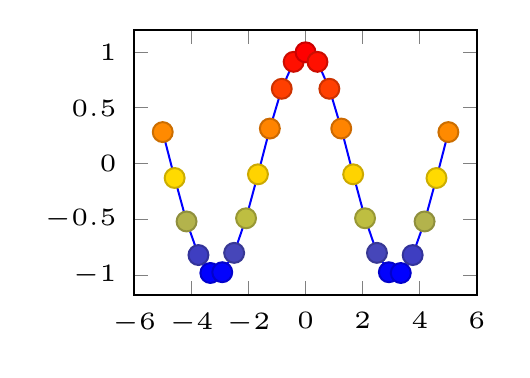
\begin{tikzpicture}[scale=1.8]
		\begin{axis}[tiny]
		\addplot+ [scatter] {cos(deg(x))};
		\end{axis}
		\end{tikzpicture}

		\captionof{figure}{A figure.}
		\label{fig:test1}
	\end{minipage}%
	\begin{minipage}{.48\textwidth}
		\centering
		
		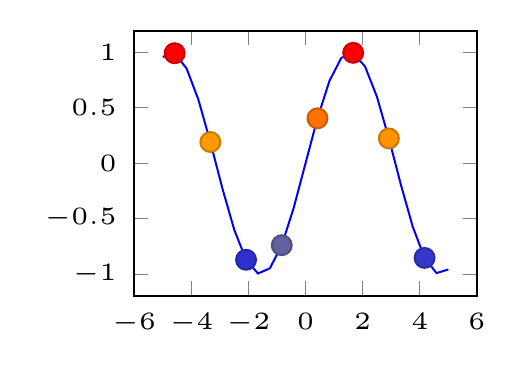
\begin{tikzpicture}[scale=1.8]
		\begin{axis}[tiny]
		\addplot+ [scatter,
		mark repeat=3,mark phase=2]
		{sin(deg(x))};
		\end{axis}
		\end{tikzpicture}
			
		\captionof{figure}{Another figure.}
		\label{fig:test2}
	\end{minipage}
\end{figure}


Fig. \ref{fig:test1} and Fig. \ref{fig:test2} represent two figures. In what follows, we draw an automaton using \LaTeX. All the sizes of elements in a drawing can be controlled.


\begin{figure}[htbp]
\begin{center}
	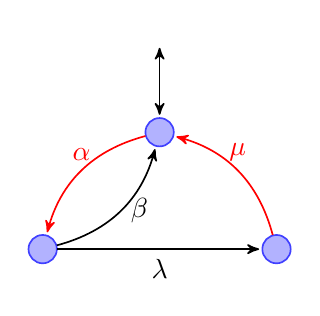
\begin{tikzpicture}
				[->,>=stealth',shorten >=1pt,auto,node distance=3.5cm,
				semithick,scale=.6,bend angle=45]
				%%%右箭头,箭头样式,自动适应,node默认间距,线条默认半粗,比例,默认弯角
				\tikzstyle{every state}=[fill=blue!30,draw=blue!75,text=black,minimum size=6mm,scale=1.5]
				%默认state样式为蓝色(0-100)填充,蓝色线条,黑色文本,最小size,比例
				%画出所有node
				\node[state,scale=0.4](0)                       {};
				%大括号内是node中的内容,(0)为该node的代号
				\node[state,scale=0.4](1) [below left of=0]     {};
				%[]内为(1)在(0)的左下位置,默认间距
				\node[state,scale=0.4](2) [below right of=0]    {};
				\node[draw=white]at(90:2)                       {}
				%一个不画出的node,由角坐标给出位置,注意这里还没有分号
				edge[<->](0);%其后可以直接定义edge,以分号结束指令
				
				
				%在node之间添加连线.第一个中括号中内容是连线的性质(颜色、弯曲方向和角度)
				%第二个括号中的内容是每条连线所附带的字母与连线的相对位置。有right\left\below\above可选
				\path 
				(0)edge [red,bend angle=30,bend right]node[above]{$\alpha$}      (1) %0到1
				(1)edge [bend angle=30,bend right]    node[right]{$\beta$}       (0)  
				(1)edge                               node[below]{$\lambda$}     (2)
				(2)edge [red,bend angle=30,bend right]node[above]{$\mu$}         (0)
				;%完整指令后以分号结束
			\end{tikzpicture}
\end{center}
\caption{This is an automaton.}
    \label{fig:my_label}
\end{figure}



\begin{figure}[htbp]
\centering
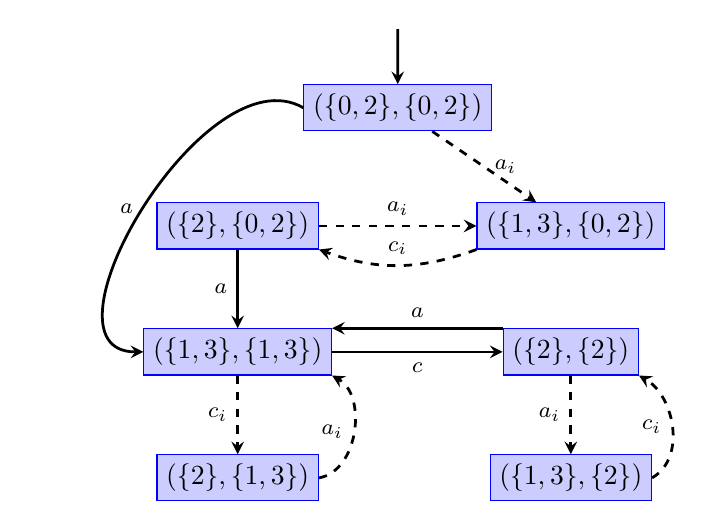
\begin{tikzpicture}[>=stealth]
	\node (state0) [draw=blue,fill=blue!20,xshift=2cm] {$(\{0,2\},\{0,2\})$};
	\node (state1) [draw=blue,fill=blue!20,left=1cm of state0.center,yshift=-1.5cm] {$(\{2\},\{0,2\})$};
    \node (state2) [draw=blue,fill=blue!20,right=1cm of state0.center,yshift=-1.5cm] {$(\{1,3\},\{0,2\})$};
    \node (state3) [draw=blue,fill=blue!20,below=1.3cm of state1.center] {$(\{1,3\},\{1,3\})$};
    \node (state4) [draw=blue,fill=blue!20,below=1.3cm of state2.center] {$(\{2\},\{2\})$};
    \node (state5) [draw=blue,fill=blue!20,below=1.3cm of state3.center] {$(\{2\},\{1,3\})$};
    \node (state6) [draw=blue,fill=blue!20,below=1.3cm of state4.center] {$(\{1,3\},\{2\})$};
    \draw[->,line width=1pt]  (2,1) -- (state0.north);
    \draw [->,line width=1pt,dashed] (state0) to node [right] {\footnotesize$a_{i}$} (state2);
	\draw [->,line width=1pt,dashed] (state1) to node [above] {\footnotesize$a_{i}$} (state2);
    \draw [->,line width=1pt,dashed] (state2.south west) to [in=340,out=200] node [above] {\footnotesize$c_{i}$} (state1.south east);
    \draw [->,line width=1pt,dashed] (state3.south) to node [left] {\footnotesize$c_{i}$} (state5.north);
	\draw [->,line width=1pt,dashed] (state5.east) to [in=330,out=10] node [left] {\footnotesize$a_{i}$} (state3.south east);
    \draw [->,line width=1pt,dashed] (state4.south) to  node [left] {\footnotesize$a_{i}$} (state6.north);
    \draw [->,line width=1pt,dashed] (state6.east) to [in=330,out=30] node [left] {\footnotesize$c_{i}$} (state4.south east);
    \draw [->,line width=1pt] (state1) to node [left] {\footnotesize$a$} (state3);
    \draw [->,line width=1pt] (state3) to node [below] {\footnotesize$c$} (state4);
    \draw [->,line width=1pt] (state4.north west) to node [above] {\footnotesize$a$} (state3.north east);
    \draw [->,line width=1pt] (state0.west) to [in=180,out=150] node [left] {\footnotesize$a$} (state3.west);
\end{tikzpicture}
\caption{Indicator automaton and verifier of the NFA in Fig. \ref{fig:my_label}}\label{indicator-NFA}
\end{figure}

\section{An example of table}
The table title is at the top of the table.

\begin{table}[htbp]	
	\centering
	\caption{A table.}
	\begin{tabular}[l]{@{}lcccccc}		
		\toprule		
		Class$^{\rm a}$ & $\gamma_1$ & $\gamma_2$$^{\rm b}$& $\langle \gamma \rangle$& $G$ & $|{ f}|$ & $\theta _{c}$ \\		
		\midrule	
		BL Lacs &5 & 36 & 7 & $-4.0$ & $1.0\times 10^{-2}$ & 10$^\circ$ \\		
		FSRQs & 5 & 40 & 11 & $-2.3$ & $0.5\times 10^{-2}$ & 14$^\circ$ \\		
		\bottomrule		
	\end{tabular}
	\label{tab:t1}
\end{table}

\begin{table}[htbp]  
\caption{Another table.}  
\begin{center}  
\begin{tabu} to 0.8\textwidth{X[c]|X[3,b]|X[2,l]|X[c]|X[3,m]|X[1,c]}  
%0.8\textwidth   为设置表格宽度  
%X[c]      表示这一列居中,所占比例为1,相当于X[1,c]  
%X[3,c]   表示这一列居中,所占比例为3,这列的宽度是X[c]列的3倍  
\hline  
$i$  &$x_i$              &$n_i$      &$i$    &$x_i$               &$n_i$\\  
\hline  
1    &0.5$\sim$0.64       &1           &8    &1.48$\sim$1.62      &53\\  
2    &0.64$\sim$0.78      &2           &9    &1.62$\sim$1.76      &25\\  
3    &0.78$\sim$0.92      &9           &10   &1.76$\sim$1.90      &19\\  
4    &0.92$\sim$1.06      &26          &11   &1.90$\sim$2.04      &16\\  
5    &1.06$\sim$1.20      &37          &12   &2.04$\sim$2.18      &3\\  
6    &1.20$\sim$1.34      &53          &13   &2.18$\sim$2.38      &1\\  
7    &1.34$\sim$1.48      &56          &     &                    & \\  
\hline  
\end{tabu}  
\end{center}  
\end{table}

\chapter{Research Method}
\section{Overview}
In this work, we will define the label categories forged as 1 $(y=1)$ and genuine as 0 $(y=0)$ for handwritten signatures, and the input reference signature image is defined as $R \in \mathbb{R}^{H\times W\times 1}$ and the query signature image is defined as $Q \in \mathbb{R}^{H\times W\times 1}$.

\begin{figure}[htbp]
  \begin{center}
      \includegraphics[scale=0.46]{figure/osvtf.jpg}
  \end{center}
  \caption{OSVTF structure Detail}
  \label{fig:osvtf}
\end{figure}

The architecture of the proposed Offline Signature Verification TransFormer (OSVTF) model for multi-scale feature fusion is shown in Fig. \ref{fig:osvtf}, which consists of five parts, namely, Backbone ($\mathcal{B}$), FPN Fusion ($\mathcal{F}$), Holistic Encoder ($\mathcal{H}$), and Conv-Module ($\mathcal{C}$), Contrast based Part Decoder ($\mathcal{P}$) five parts. In the model we will input a pair of signature image samples $\mathbf{I}_r$ and $\mathbf{I}_q$, the initial input image goes through Backbone with shared weights (ResNet-50 \cite{14} is used as an example in Fig. \ref{fig:osvtf}) to get the multi-scale feature map set $\mathcal{B}(\mathbf{I}_r),\mathcal{B}(\mathbf{I}_q)$, and then the different scale feature maps are fused through FPN Fusion module, and the output of multi-scale fusion feature maps $\mathbf{F}_r^\mathcal{F},\mathbf{F}_q^\mathcal{F}$. Then it enters the Holistic Encoder with shared weights to get the holistic flat features $f_r^\mathcal{H},f_q^\mathcal{H}$ and patch embeddings $\boldsymbol{x}_r^\mathcal{H}=[x_r^{\mathcal{H}_1 }, \cdots, x_r^{\mathcal{H}_N} ]$ and $\boldsymbol{x}_q^\mathcal{H} = [ x_q^{\mathcal{H}_1}, \cdots, x_q^{\mathcal{H}_N} ]$. To further integrate the feature maps, the above patch embeddings are reshaped to a 2D shape, and its outputs $\mathbf{F}_r^\mathcal{C}, \mathbf{F}_q^\mathcal{C}$ are obtained after the Convolutional Module (Conv-Module) with shared weights, and they will go directly to the Contrast based Part Decoder to obtain the cross-attention contrast part flat features $f_r^\mathcal{P},f_q^\mathcal{P}$. In the final prediction stage, Global Average Pooling (GAP) operation is performed on $\mathbf{F}_r^\mathcal{F},\mathbf{F}_q^\mathcal{F}$ and $\mathbf{F}_r^\mathcal{C},\mathbf{F}_q^\mathcal{C}$ to obtain the multiscale fusion flat features $f_r^\mathcal{F},f_q^\mathcal{F}$ and convolution flat features $f_r^\mathcal{C},f_q^\mathcal{C}$. The total feature vector $f_r=[f_r^\mathcal{F},f_r^\mathcal{H},f_r^\mathcal{C},f_r^\mathcal{P} ]$ and $f_q=[f_q^\mathcal{F},f_q^\mathcal{H},f_q^\mathcal{C},f_q^\mathcal{P} ]$ of the OSVTF are obtained by splicing all the flat features, and the judgment of whether $\mathbf{I}_q$ is forged or not will be made based on $f_r$ and $f_q$. Next, Backbone, FPN Fusion, Holistic Encoder, Conv-Module and Contrast based Part Decoder structures will be analyzed in depth.

\section{Backbone}

In the Backbone section an architecture of CNN will be adopted that discards Average Global Pooling and Fully Connected Layers in the output section.Most of the CNN architecture consists of a convolutional layer in the input section and four defined convolutional layers, as shown in Fig. 3 for example in ResNet-50 \cite{14}, where each layer consists of a number of bottleneck blocks. A single bottleneck block consists of two convolutional 2D layers with convolutional kernels of ($1\times 1 \to 3\times 3 \to 1\times 1$), and this arrangement mainly has the following purposes: 1. Reduce the feature dimensions to achieve the purpose of improving the computational efficiency; 2. The intermediate $3\times 3$ convolution extracts the local spatial features such as strokes, edges, etc., in the lower dimensional space has the ability to maintain the sensory field while reducing the redundancy, and this reduces the number of channels before expanding to the input, and then the number of channels is expanded to the input, and the number of channels is reduced. This first reduces the number of expression channels and then expands to the input expression channels to find better feature learning parameters in the bottomleneck, which has a better feature abstraction and expression ability; 3. In the actual operation, it can be paired with the identity skip connection to quickly propagate the gradient to avoid gradient disappearance, and at the same time, such a design makes the number of intermediate parameters and the burden of computation greatly reduced, and it can stack more layers. At the same time, this design can greatly reduce the number of intermediate parameters and computational burden, and can stack more layers, such as ResNet-101, to promote the training of deeper networks; 4. This modular design has the advantage of easy fine-tuning of the convolutional parameters, and the number of intermediate channels can be adjusted according to the environment, so as to control the balance of performance and efficiency. In addition, ResNet series network introduces residual connection, which solves the problem of missing features after deep convolutional operation of the image. Residual connection is introduced in each bottomleneck block, which accumulates the feature map of the input part with the output of the bottomleneck, which can reduce the problem of feature loss after a certain number of convolutional layer operations to a certain extent.

Assume that the input feature map $ \mathbf{I} \in \mathbb{ R }^{ H\times W\times C } $ of the convolutional layer, the output feature map $\boldsymbol{z} \in \mathbb{ R }^{ H'\times W'\times C' }$, the convolutional kernel size of the convolutional 2D layer $K\times K$ (the convolutional kernel weight $ \tilde{\mathbf{W}} \in \mathbb{ R }^{ K\times K\times C\times C' } $, the padding $\tilde{P}$, the step size $\tilde{S}$, and the bias term $\tilde{b}$. For the $c'$-th output channel of the feature map, the pixel point with spatial location $(i,j)$ is calculated as eq. \ref{eq1}.

\begin{equation}
\label{eq1}
  \boldsymbol{z}(i, j, c') = \sum^{C'}_{c=1} \sum^K_{u=1} \sum^K_{v=1} = \tilde{\mathbf{W}}_{u, v, c, c'} \cdot \mathbf{I}(i\cdot \tilde{S}+u-\tilde{P}, j\cdot \tilde{S}+v - \tilde{P}, c) + \tilde{\mathbf{b}}_{c'}
\end{equation}

In addition, in each bottleneck block, except for the last $1\times 1$ convolutional 2D layer which is followed only by the BatchNorm (BN) \cite{16} operation, each convolutional 2D layer will be followed immediately by the BN and ReLU activation function \cite{29} operation (Conv2D$\to$BN$\to$ReLU), and the spatial location $(i,j,c')$ after the BN and ReLU activation function is the pixel point values are as eq. \ref{eq2}.

\begin{equation}
\label{eq2}
  \hat{\boldsymbol{z}}(i, j, c') = \max \left( 0, \gamma_c \frac{\boldsymbol{z}(c', i, j) - \mu'_c}{\sqrt{\sigma^2_{c'}+\epsilon}}+\beta_{c'} \right)
\end{equation}

Where $\mu,\sigma^2$ are the mean and variance of the feature statistics of the $c'$ channel plane in the batch multi-channel feature maps output from the convolutional 2D layer, and $\gamma, \beta$ are the learnable scaling and translation parameters. This shows that the idea of the BN operation is to normalize a certain batch of data, which has the effect of improving the convergence speed when training the model parameters. In each bottomleneck block operation, a cumulative residual operation is performed on the feature maps after three convolutional 2D operations, i.e., the feature maps input to the bottomleneck block are added to the feature maps output from the three convolutional 2D operations, which are then passed to the next bottomleneck block. At the same time, each layer of the backbone operation will be followed by a downsampling operation as a way to reduce the redundant features on the multi-channel feature map, which will be taken as Max Pooling 2D in order to equate the downsampling operation \cite{14}. The above residual linking approach can ensure that the feature map retains certain original image features after the convolution operation, so the ResNet family of networks is most suitable as the backbone of the depth model to extract the image multi-channel feature map.

The backbone is taken mainly to extract the image multi-scale feature maps, so the different scale feature maps of each layer except the input convolutional layer are included in the final output as eq. \ref{eq3}.

\begin{equation}
\label{eq3}
  \mathcal{B}(\mathbf{I}) = \{ \mathbf{F}^{\mathcal{B}(1)}, \mathbf{F}^{\mathcal{B}(2)}, \mathbf{F}^{\mathcal{B}(3)}, \mathbf{F}^{\mathcal{B}(4)} \}
\end{equation}

where the multi-channel feature map $\mathbf{F}^\mathcal{B}(i) \in \mathbb{R}^{\frac{H}{2^{i+1}} \times \frac{W}{2^{i+1}} \times \frac{C}{2^{i-1}}},(i=1,2,3,4)$ for each scale, H,W,C denote the width, height and the number of channels of the output feature maps of layer 1, and $C=256$ when the backbone is ResNet-50), and each layer of the feature map has a twofold relationship between the channels and dimensions.

\section{FPN Fusion}

In order to be able to effectively utilize the multi-scale feature maps extracted by backbone, the Feature Pyramid Network Fusion (FPN Fusion) module is used in order to fuse feature maps at different scales, which adopts the model architecture of FPN-Style \cite{23}, as shown in Figure \ref{fig:fpn}.

\begin{figure}[htbp]
  \begin{center}
      \includegraphics[scale=0.45]{figure/fpn.jpg}
  \end{center}
  \caption{FPN Fusion module structure}
  \label{fig:fpn}
\end{figure}

Where the bottom-up process is the process of backbone inference to obtain different scales of feature maps. In bottom-down, for each layer of feature maps, a convolutional 2D layer with a convolutional kernel of $1\times 1$ will be taken for mapping, which maps the feature maps with different number of channels at each scale to the same feature dimensions, and achieves the operation of dimensionality reduction to a certain extent, so as to accelerate the speed of model inference. At the same time, $\mathbf{F}^{\mathcal{B}(2)} ,\mathbf{F}^{\mathcal{B}(3)} ,\mathbf{F}^{\mathcal{B}(4)}$ are up-sampled to increase the size to the same size as $\mathbf{F}^{\mathcal{B}(1)}$, and then fused according to the fusion method in order to get the multi-scale fusion feature map. Bilinear interpolation \cite{18} is adopted in the up-sampling process, for the lth layer feature map up-sampling output $\mathbf{F}^{\mathcal{B}(l)}$, the value of spatial location $(i',j',c)$ is calculated as eq. \ref{eq4}.

\begin{equation}
\label{eq4}
  \begin{aligned}
    \mbox{Up}(\mathbf{F}^{\mathcal{B}(l)})(i', j', c) &= (1-\delta_i)(1-\delta_j)\cdot \mathbf{F}^{\mathcal{B}(l)}(i, j, c)\\
    &+\delta_i(1-\delta_j)\cdot \mathbf{F}^{\mathcal{B}(l)}(i+1, j, c) \\
    &+(1-\delta_i)\delta_j\cdot \mathbf{F}^{\mathcal{B}(l)}(i, j+1, c) \\
    &+\delta_i \delta_j \cdot \mathbf{F}^{\mathcal{B}(l)}(i+1, j+1, c)
  \end{aligned}
\end{equation}

where $\delta_i=\frac{i'}{s_i} - \lfloor \frac{i'}{s_i} \rfloor, \delta_j = \frac{j'}{s_j} - \lfloor \frac{j'}{s_j} \rfloor$ denote fractional portions of the value in the direction of the width and the height, $s_i,s_j$ denote the magnification $(s_i = s_j = 2)$, and $\lfloor \cdot \rfloor$ denotes the value of the integer part. This up-sampling method can well preserve the original feature ground structure while introducing a smooth transition as shown in Fig. \ref{fig:bilinear}. 

\begin{figure}[htbp]
  \centering
  \includegraphics[scale=0.8]{figure/bilinear.png}
  \caption{Bilinear interpolation example}
  \label{fig:bilinear}
\end{figure}

Each up-sampled pixel point will be weighted according to the original feature map pixel points, which not only retains the structural scale of the original feature map, but at the same time makes the transition between pixel points smoother, and to a certain extent, it can reflect the effect of different scales on the image feature points, for example, the features of a certain stroke will be enlarged.

After each scale feature map is sampled on the ground by bilinear interpolation, it will be fused according to three ways: accumulation, weighted average, and channel splicing. The first way is the traditional FPN-Style approach, which directly performs the accumulation operation on the downscaled multi-scale feature maps directly, similar to the residual link mentioned above. The design idea of the second way is to be able to ensure that the signature images of different scenarios can have a certain learning ability, by setting the proportion of weights to be able to pay more attention to the features of a certain scale, and the default is to take all equal weights. The third way is to splice in the channel dimension, followed by a convolutional kernel $1\times 1$ convolutional 2D operation, this method can maximize the retention of all scales of features, but may lead to the model computational overhead is too large, resulting in slower convergence of the model.

After fusing the multi-scale feature map, it will finally go through a convolutional 2D layer with a convolutional kernel $3\times 3$ to smooth out the checkerboard artifacts brought about by the up-sampling process, and finally output the multi-scale fused feature map $\mathbf{F}^\mathcal{F} = \mathcal{F}(\mathcal{B}(\mathbf{I})) \in \mathbb{R}^{\frac{H}{4}\times \frac{W}{4}\times C}$.

\section{Holistic Encoder}

\begin{figure}[H]
  \begin{center}
      \includegraphics[scale=0.6]{figure/encoder.jpg}
  \end{center}
  \caption{Holistic Encoder structure}
  \label{fig:encoder}
\end{figure}

The Holistic Encoder is designed with reference to Vision Transformer (ViT) \cite{4} The architecture is shown in Fig. 6. swing embeddings \cite{24} are adopted in the input stage instead of the previous chunking operation, where chunking and mapping are performed on the input multiscale fusion feature maps according to the set window size $P\times P$ and step size S , the patch embeddings are obtained and then flattened to be used as feature vectors $[\overline{x}^{\mathcal{H}_1},\overline{x}^{\mathcal{H}_2},\cdots ,\overline{x}^{\mathcal{H}_N}] \in \mathbb{R}^{N\times D}$, where D denotes the number of mapped feature dimensions, and the vector length, $N$, is computed as eq. \ref{eq5}.


\begin{equation}
\label{eq5}
  N=\lfloor \frac{H/4-P+S}{S}\rfloor \times \lfloor \frac{W/4-P+S}{S}\rfloor
\end{equation}

Splicing a learnable weight $\overline{f}^{\mathcal{H}}\in \mathbb{R}^D$ defined as a class token in swing embeddings, i.e., the feature vector of the input Transformer Encoder Layer is $\overline{\boldsymbol{x}}^\mathcal{H}=[\overline{f}^\mathcal{H},\overline{x}^{\mathcal{H}_1},\overline{x}^{\mathcal{H}_2},\cdots ,\overline{x}^{\mathcal{H}_N} ] \in \mathbb{R}^{(N+1)\times D}$. Due to the flattening operation performed on the feature map, positional embeddings \cite{36} need to be accumulated on the feature vectors as a way to make the feature vectors contain information about their positions on the multiscale fused feature map.

After swing embeddings, the feature vector $\overline{\boldsymbol{x}}^\mathcal{H}$ enters the Transformer Encoder Layer for attention feature computation. Where Transformer Encoder Layer is formed by $L$ stacks as shown in Fig. \ref{fig:mhsa}.

\begin{figure}[H]
  \begin{center}
      \includegraphics[scale=0.55]{figure/mhsa.jpg}
  \end{center}
  \caption{Transformer Encoder Layer structure}
  \label{fig:mhsa}
\end{figure}

Each Transformer Encoder Layer consists of a Multi-Head Self Attention $\to$ Add \& LN and Feed Forward Network $\to$ Add \& LN, where Add \& LN denotes residual linking and LayerNormalization (LN) \cite{1}. The input feature vectors first enter Multi-Head Self Attention (MHSA) in order to perform the computation of the attention mechanism, which is essentially Multi-Head Attention (MHA) except that the sources before the mapping of $\boldsymbol{X}_\text{q} \in \mathbb{R}^{N\times d_q}$ and $\boldsymbol{X}_\text{k}, \boldsymbol{X}_\text{v} \in \mathbb{R}^{N\times d_k }$ in the operations are The same, i.e., the input feature vectors will be simultaneously entered into the linear mapping layer of each head for dimensionality reduction, thus generating the query vector $\boldsymbol{X}_\text{q}$, the key vector $\boldsymbol{X}_\text{k}$, the value vector $X_v$, and $d_q = d_k$. where the attention mechanism is divided into multiple head computations in order to conserve the computational resources, and the feature vectors will be entered into the three linear layers of the $M$ heads in order to be dimensionality reduced for mapping, thus achieving the attention computation in parallel, and the final splice and linear layer mapping will input vectors with the same feature dimensions, so the output vector shape of MHSA is the same as the input vector shape. The attention feature vectors of each head in MHSA are computed by taking scaled dot product attention \cite{36} with the following eq. \ref{eq6}.

\begin{equation}
\label{eq6}
  \text{Attn}(\boldsymbol{X}_\text{v}, \boldsymbol{X}_\text{k}, \boldsymbol{X}_\text{v}) = \text{Softmax} \left( \frac{\boldsymbol{X}_\text{q}\boldsymbol{X}_\text{k}^\mathrm{T}}{\sqrt{d_k}} \right)\cdot \boldsymbol{X}_\text{v}
\end{equation}

In this case, there is a soft query relationship between $\boldsymbol{X}_\text{q}, \boldsymbol{X}_\text{k}$ and $\boldsymbol{X}_\text{v}$. Instead of selecting a specific key-value pair for each query, all key-values are weighted and averaged, and the weights are computed by the similarity between $\boldsymbol{X}_\text{q}$ and $\boldsymbol{X}_\text{k}$. each feature token of $\boldsymbol{X}_\text{q}$ establishes a relevance distribution, i.e., a Softmax \cite{37} of attention weights, based on which the values of $\boldsymbol{X}_\text{v}$ are weighted and fused. The advantage of this mechanism is that it can focus on multiple relevant tokens at the same time, which enables the model to more fully model the contextual information, for example, the $(i, j)$ position of attention weight indicates the weight of $i$-th position of $\boldsymbol{X}_\text{q}$ on the $j$-th position of $\boldsymbol{X}_\text{k}$, the larger the value of this weight, the stronger the contextual relationship of the query at the $i$-th position to the key at $j$-th position, and conversely the smaller the value, the relationship is very small. According to this attention weight, multiplying $\boldsymbol{X}_\text{v}$ again will further amplify the features in the place where the attention weight of its own vector is high, and the attention information will be included between tokens, so as to achieve that each token owns its own global information, and can more effectively utilize the important features and ignore the useless features, and will more effectively pay attention to the part of the brush strokes in the image of the handwritten signature, ignoring the blank part. The resulting MHSA output of a single Transformer Encoder Layer is as eq. \ref{eq7}.

\begin{equation}
\label{eq7}
\text{MHSA}(\overline{\boldsymbol{x}}^\mathcal{H},\mathbf{T},\mathbf{L}) =
\begin{bmatrix}
  \text{Attn}(\overline{\boldsymbol{x}}^\mathcal{H} \mathbf{T}_{1,1},\overline{\boldsymbol{x}}^\mathcal{H} \mathbf{T}_{1,2},\overline{\boldsymbol{x}}^\mathcal{H} \mathbf{T}_{1,3}) \\
  \text{Attn}(\overline{\boldsymbol{x}}^\mathcal{H} \mathbf{T}_{2,1},\overline{\boldsymbol{x}}^\mathcal{H} \mathbf{T}_{2,2},\overline{\boldsymbol{x}}^\mathcal{H} \mathbf{T}_{2,3}) \\
  \cdots \\
  \text{Attn}(\overline{\boldsymbol{x}}^\mathcal{H} \mathbf{T}_{m,1},\overline{\boldsymbol{x}}^\mathcal{H} \mathbf{T}_{m,2},\overline{\boldsymbol{x}}^\mathcal{H} \mathbf{T}_{m,3}) \\
\end{bmatrix}^{\mathrm{T}}
\cdot \mathbf{L} 
\end{equation}

where $\mathbf{T}_l \in \mathbb{R}^{M\times 3\times d_k\times d_k' }$ denotes the linear mapping layer weights in the input phase of the MHSA, $\mathbf{L} \in \mathbb{R}^{d_k\times d_k' }$ denotes the weights of the final linear mapping layer in the MHSA, and $d_k'$ denotes the number of feature dimensions of each head $\boldsymbol{X}_\text{q}, \boldsymbol{X}_\text{k}$ and $\boldsymbol{X}_\text{v}$, and thus must satisfy $d_k=M\times d_k'$.

Matrix multiplication with larger dimensions is performed in the MHSA section, and in order to reduce the risk of gradient explosion or vanishing, and also to reduce the missing information of the original feature vectors, a residual link and an LN layer follow immediately after the MHSA.The main role of the LN layer is to normalize the feature vectors at each position, thus speeding up the convergence of the model as well as improving the model stability. Unlike the mean and variance of the BN, the mean and variance of the LN are derived from the current feature dimensions on which they are calculated as eq. \ref{eq8}.

\begin{equation}
\label{eq8}
\begin{aligned}
  \mu &= \frac{1}{d_k}\sum^{d_k}_d \text{MHSA}(\overline{\boldsymbol{x}}^\mathcal{H}, \mathbf{T}, \mathbf{L})_d \\
  \sigma^2 &= \frac{1}{d_k}\sum^{d_k}_d \left( \text{MHSA}(\overline{\boldsymbol{x}}^\mathcal{H}, \mathbf{T}, \mathbf{L})_d - \mu \right)^2
\end{aligned}
\end{equation}

where $\text{MHSA}(\overline{\boldsymbol{x}}^\mathcal{H},\mathbf{T},\mathbf{L})_d$ denotes the dth feature dimension of the MHSA output feature vector. The subsequent normalization operation is the same as in the BN layer, and the entire MHSA$\to$Add \& LN output is computed as eq. \ref{eq9}.

\begin{equation}
\label{eq9}
  \hat{\text{MHSA}}(\overline{\boldsymbol{x}}^\mathcal{H}, \mathbf{T}, \mathbf{L}) = \gamma \cdot \left( \frac{\text{MHSA}(\overline{\boldsymbol{x}}^\mathcal{H}, \mathbf{T}, \mathbf{L}) - \mu}{\sqrt{\sigma^2+\epsilon}} + \mathcal{E}_{l-1} \right) + \beta
\end{equation}

Where $\mathcal{E}_{l-1}$ denotes the output of the previous Transformer Encoder Layer, if $l=1$, then $\mathcal{E}_{l-1}=\overline{\boldsymbol{x}}^\mathcal{H}$. After the attention computation, Feed Forward Network (FFN) is introduced to enhance the overall model to model the complex patterns \cite{8}, and the whole FFN is computed as eq. \ref{eq10}:

\begin{equation}
\label{eq10}
  \text{FFN}(\hat{\text{MHSA}}(\overline{\boldsymbol{x}}^\mathcal{H}, \mathbf{T}, \mathbf{L})) = \mathcal{G}(\hat{\text{MHSA}}(\overline{\boldsymbol{x}}^\mathcal{H}, \mathbf{T}, \mathbf{L})\mathbf{W}_1 + \mathbf{b}_1)\mathbf{W}_2 + \mathbf{b}_2
\end{equation}

Where $\mathbf{W}_1\in \mathbb{R}^{D\times d_{ff}}, b_1\in \mathbb{R}^{d_{ff}}$ denotes the weight and bias of the first linear layer in the FFN, and $\mathbf{W}_2\in \mathbb{R}^{d_{ff}\times D}, \mathbf{b}_2\in \mathbb{R}^D$ denotes the weight and bias of the second prior layer in the FFN, $\mathcal{G}$ denotes the GeLU function \cite{15}. the GeLU function and the ReLU function act similarly as the activation function that performs the nonlinear transformation. The entire FFN is a nonlinear transformation of the model, which complements the global interaction mechanism of Attention to jointly build a powerful context-aware representation. Subsequently followed by Add \& LN to supplement the feature information and accelerate the model convergence, each subsequent layer of Transformer Encoder Layer is a stacking effect to deepen the Attention weight of the feature vectors, and the output of the whole Holistic Encoder is $\{f^\mathcal{H}, \boldsymbol{x}^\mathcal{H} \} = \mathcal{H}(F^\mathcal{F}),f^H\in \mathbb{R}^D,x^\mathcal{H} \in R^{N\times D}$.

\section{Conv-Module}

The image features are subjected to feature learning by Holistic Encoder capturing the relative position information of the elements in the sequence, but it has the limitation of learning absolute position information. The signature verification task needs to be accurate to the stroke position information (e.g., stroke order, local structural differences), so after this in order to enhance some small portion of the image features, the output $\boldsymbol{x}^\mathcal{H}$ of the patch token of the Holistic Encoder is rearranged, and the flattened token is reconverted into a 2D shape $\mathbf{F}^\mathcal{H} \in \mathbb{R}^{h\times w\times D}$ to perform a convolution operation, where $h = \lfloor \frac{H/4-P+S}{S}\rfloor,w = \lfloor \frac{W/4-P+S}{S}\rfloor $. This module introduces the convolution operation to reprocess the patch features output from the Transformer encoder to enhance the position-awareness. In the Conv-Module architecture, the Conv design of TransOSV \cite{41} is referenced, and the number of output channels of the intermediate convolutional 2D layer is adjusted to increase the downsampling operation according to the style of previous CNNs, as shown in Table \ref{tab:conv}.


\begin{table}[htbp]
\caption{Conv-Module layers information}  
\begin{center}
\begin{tabu} to 0.8\textwidth{X[3, c]X[3, c]X[3, c]}  
%0.8\textwidth   为设置表格宽度  
%X[c]      表示这一列居中,所占比例为1,相当于X[1,c]  
%X[3,c]   表示这一列居中,所占比例为3,这列的宽度是X[c]列的3倍  
\toprule
Layer & Kernel Size & Output feature map\\
\midrule
Conv2D + ReLU & $3\times 3$ & $h\times w\times d_\mathcal{C}$ \\ 
Conv2D + ReLU & $3\times 3$ & $h\times w\times d_\mathcal{C}$ \\ 
Max Pooling 2D & $2\times 2$ & $\frac{h}{2}\times \frac{w}{2}\times d_\mathcal{C}$ \\ 
Conv2D + ReLU & $3\times 3$ & $\frac{h}{2}\times \frac{w}{2}\times \frac{d_\mathcal{C}}{2}$ \\ 
Conv2D + ReLU & $3\times 3$ & $\frac{h}{2}\times \frac{w}{2}\times \frac{d_\mathcal{C}}{2}$ \\ 
Conv2D + ReLU & $3\times 3$ & $\frac{h}{4}\times \frac{w}{4}\times \frac{d_\mathcal{C}}{2}$ \\ 
\bottomrule
\end{tabu}
\end{center}
\label{tab:conv}
\end{table}

Different from the traditional CNN with gradually more channels, the overall downsampling operation thinking is adopted here, and certain downsampling operations are performed on the patch features to abstractly express the local features of the feature map on the basis of integrating the local detail features, with the purpose of enhancing the generalization ability and robustness of the model. This operation is added on the basis of backbone and FPN Fusion to further strengthen the model's ability to perceive the local features of the image, strengthen the focus on the key local regions of the signature, and filter the background interference at the same time. In the Conv-Module module, each Conv2D layer operation is the same as the Conv2D layer operation in backbone, which takes the combination of Conv2D+ReLU, and after two Conv2D+ReLUs a downsampling operation, i.e., Max Pooling 2D operation, will be performed to integrate the feature maps and eliminate the non-important parts of the features to integrate and eliminate non-important parts of the feature map and enhance feature expressiveness.

In the model training process, the output $\mathbf{F}^\mathcal{C} = \mathcal{C}(\mathbf{F}^\mathcal{H} ) \in \mathbb{R}^{h'\times w'\times d_C' }$ of the Conv-Module will undergo a Global Average Pooling (GAP) operation while entering the Contrast based Part Decoder to globally sample the feature maps of the output of the Conv-Module. The feature maps of the Conv-Module are globally sampled to obtain a flat local convolutional feature $f^\mathcal{C}$ to complete the corresponding feature extraction in the training and inference process.

\section{Contrast based Part Decoder}

\begin{figure}[H]
  \centering
      \includegraphics[scale=0.45]{figure/decoder.jpg}
  \caption{Contrast based Part Decoder structure}
  \label{fig:decoder}
\end{figure}

This part is an improvement on TransOSV's Contrast based Part Decoder \cite{41} for parallel computation of Cross-Attention, which references the multi-head attention computation mechanism of MHSA in Holistic Encoder. Similar to the Holistic Encoder part, the feature maps of references and query are mapped to the $d_\mathcal{P}$ feature dimension in the input phase, followed by flattening and addition of a learnable weight $f_r^{\mathcal{P}_{cls}},f_q^{\mathcal{P}_{cls}} \in \mathbb{R}^D$, also defined as a class token, i.e., the input part is obtained as a pair of flattened feature map vectors $\boldsymbol{x}_r^\mathcal{P} = [f_r^{\mathcal{P}_{cls}}, x_r^{\mathcal{P}_1},\cdots ,x_r^{\mathcal{P}_{h' w' }} ]$, $\boldsymbol{x}_q^\mathcal{P}=[f_q^{\mathcal{P}_{cls}},x_q^{\mathcal{P}_1},\cdots,x_q^{\mathcal{P}_{h'w'} } ] \in \mathbb{R}^{h' \times w' \times (D+1)}$. Subsequently, MHSA operations are performed on $\boldsymbol{x}_r^\mathcal{P},\boldsymbol{x}_q^\mathcal{P}$ to take out the class token $\overline{f}_r^{\mathcal{P}_{cls}},\overline{f}_q^{\mathcal{P}_{cls}} \in \mathbb{R}^D$ of their respective output eigenvectors as the query matrix cross-input Cross Multi-Head Attention (CMHA).The structure of CMHA is shown in Figure 8-b shown, differs from MHA in that only the query matrix and key matrix are generated to compute their cross-attention weights $\boldsymbol{\alpha}_r,\boldsymbol{\alpha}_q$, and the final concat is replaced with a weighted average to handle the attention weights of multiple heads. For a single CMHA the output cross-attention weight $\boldsymbol{\alpha}$ is calculated as eq. \ref{eq11}.

\begin{equation}
\label{eq11}
  \boldsymbol{\alpha}= \frac{1}{M}\sum^M_{m=1} \text{Softmax}\left( \frac{\boldsymbol{X}_\text{q}\mathbf{T}^\mathcal{P}_{m, 1}\cdot (\boldsymbol{X}_\text{k}\mathbf{T}^\mathcal{P}_{m, 2})^\mathrm{T} }{\sqrt{d_\mathcal{P}'}} \right)
\end{equation}

where $\boldsymbol{X}_\text{q},\boldsymbol{X}_k$ denote the input query and key vectors, $\mathbf{T}^\mathcal{P} \in \mathbb{R}^{M\times 2\times D\times d_k′}$ denotes the linear mapping layer weights of the input part of the CMHA. The resulting $\boldsymbol{\alpha}_r,\boldsymbol{\alpha}_q$ computation process is as eq. \ref{eq12}.

\begin{equation}
\label{eq12}
\begin{aligned}
  \boldsymbol{\alpha}_r = \frac{1}{M}\sum^M_{m=1} \text{Softmax}\left( \frac{\overline{f}_q^{\mathcal{P}_{cls}}\mathbf{T}^\mathcal{P}_{m, 1}\cdot (\boldsymbol{x}_r^\mathcal{P}\mathbf{T}^\mathcal{P}_{m, 2})^\mathrm{T} }{\sqrt{d_\mathcal{P}'}} \right) \\
  \boldsymbol{\alpha}_q = \frac{1}{M}\sum^M_{m=1} \text{Softmax}\left( \frac{\overline{f}_r^{\mathcal{P}_{cls}}\mathbf{T}^\mathcal{P}_{m, 1}\cdot (\boldsymbol{x}_q^\mathcal{P}\mathbf{T}^\mathcal{P}_{m, 2})^\mathrm{T} }{\sqrt{d_\mathcal{P}'}} \right) \\
\end{aligned}
\end{equation}

Perform a weight-sum operation on the attention weights and the mapped flat feature vector $\overline{\boldsymbol{x}}_r^\mathcal{P},\overline{\boldsymbol{x}}_r^\mathcal{P}\in \mathbb{R}^{h'\times w'\times d_\mathcal{P}}$, and fuse to generate the flat feature $\overline{f}_r^P,\overline{f}_q^P\in \mathbb{R}^{d_P}$ with cross-attention weights. Its after FFN to get the flat feature $\overline{f}_r^\mathcal{P},\overline{f}_q^\mathcal{P}\in \mathbb{R}^{d_P}$ of cross attention of decoder, the whole computation process is as eq. \ref{eq13}.

\begin{equation}
\label{eq13}
  \{f_r^\mathcal{P},f_q^\mathcal{P},\boldsymbol{\alpha}_r,\boldsymbol{\alpha}_q \}=\mathcal{P}(F_r^\mathcal{C},F_q^\mathcal{C} )
\end{equation}

This Contrast based Part Decoder, which is similar to the structure of Transformer Decoder \cite{36}, facilitates the generation of local feature information that distinguishes between genuine and forged signatures, and emphasizes the feature relationship between a pair of data samples, enhancing the model's learning of the features between a pair of data in a sample. During the training process, the output cross-attention weights $\boldsymbol{\alpha}_r,\boldsymbol{\alpha}_q$ are computed with sparsity loss to force the distribution of cross-attention weights to be centralized, avoiding averaging in order to fail to pay attention to the sensitive part of forged signatures.

\section{Loss Funcion}

\subsection{Euclidean Distance}

OSVTF is a model architecture similar to twin networks, this style emphasizes that the model is a two-flow form of shared weights and the overall purpose is to compare the gap between the two, so it will be based on the similarity of the input two features in order to design the loss function. In this work, Euclidean Distance \cite{5} will be taken in order to be used as a similarity calculation for a pair of feature samples, assuming that a pair of features $f_r,f_q$ is input and the formula for calculating the distance between them is as eq. \ref{eq14}.

\begin{equation}
\label{eq14}
  \mathcal{D}(f_r, f_q) = ||f_r - f_q||_2=\sqrt{\sum_{d=1}(f^{(d)}_r - f^{(d)}_q)^2}
\end{equation}

\subsection{Focal Contrast Loss}

In the handwritten signature sample data processing stage, the handwritten signature of the writer will be paired with the pairing operation that will not be repeated between the two, for example, the BHSig-B \cite{3} dataset contains a total of 100 writers' handwritten signature images, in which each writer owns 24 genuine signature images ($y=0$) and 30 forged signature images ($y=1$), the genuine signature images are used as the reference signature, forged signature and real signature together as query signature, which will generate 276 pairs of positive samples and 720 pairs of negative samples. Thus each writer has a total of 996 data sample pairs, in which the ratio between positive and negative sample pairs is not close to 50:50, so the number of positive and negative samples is not balanced and belongs to the category of hard samples \cite{33}. 

The loss function of similarity of comparison samples used for binary classification in earlier algorithms and models is Contrast Loss \cite{10}, which is calculated as eq. \ref{eq15}.

\begin{equation}
\label{eq15}
  \mathcal{L}_c (f_r,f_q ) = (1 - y)\cdot \mathcal{D}(f_r,f_q)^2 + y\cdot \max⁡(m - \mathcal{D}(f_r,f_q),0)^2 
\end{equation}

Where $m$ denotes the boundary value, i.e., the distance that forged samples should be kept at least. For the sample pair of $y=0$, it is directly used as the loss value to make the model parameter learning on the real sample pairs of features more similar; on the contrary $y=1$, if the feature distance between the reference and query is less than $m$, $(m - \mathcal{D}(f_r,f_q ))^2$ is used as the loss value to make the model for the forged signature pairs of features is not less than $m$. However, this kind of loss can't be dynamically emphasized on the hard samples and is prone to model parameter overfitting problems. In order to reduce the risk of overfitting, a boundary value is also introduced for the genuine sample pairs to reduce the unnecessary contraction between the genuine pairs, i.e., the Double-Margin loss \cite{25} is calculated as eq. \ref{eq16}.

\begin{equation}
\label{eq16}
\begin{aligned}
  \mathcal{L}_{dm} (f_r,f_q ) &= (1-y)\cdot \max(\mathcal{D}(f_r,f_q )-n,0)^2 \\
  &+ y\cdot \max⁡(m-\mathcal{D}(f_r,f_q),0)^2
\end{aligned}  
\end{equation}

where the two boundary values m>n, penalize the case where the distance exceeds n for the genuine sample pairs, and promote the case where the distance is greater than m for the forged sample pairs. Although double margin optimizes the problem of easy overfitting by contrast loss to a certain extent, in the case of two pairs of sample data $\{r,q_1 \},\{r,q_2\}$ and $y=1$ In the case, the distance between the two sample pairs is calculated by OSVTF, if $\mathcal{D}(f_r,f_{q_1}) >> \mathcal{D}(f_r,f_{q_2}) > n $, then the loss function should give a greater loss to ${r,q_1}$, but $\mathcal{L}_{dm}$ will treat the two sample pairs equally, and the notion of dynamic weighting is introduced in TransOSV, named Focal Contrast Loss \cite{41}, which is calculated as eq. \ref{eq17}.

\begin{equation}
\label{eq17}
\begin{aligned}
  \mathcal{L}_{fc}(f_r,f_q ) &= (1 - y)\cdot \sigma(\overline{K}(\mathcal{D}(f_r,f_q )-\alpha_1 ))\cdot \max⁡(\mathcal{D}(f_r,f_q)-n,0)^2 \\
  &+ y\cdot \sigma(\overline{V} (\alpha_2 - \mathcal{D}(f_r,f_q))\cdot \max⁡(m - \mathcal{D}(f_r,f_q ))^2 \\
\end{aligned}
\end{equation}

where $\sigma(\boldsymbol{z})=\frac{1}{1+e^{-\boldsymbol{z}}}$, denotes the Sigmoid activation function \cite{26}, which is used to dynamically generate the weights; $\alpha_1,\alpha_2$ are the two margin values; $\overline{K},\overline{V}$ denote the scaling factors, which are used to regulate the scaling factor of the response strength of hard samples. When the label of the sample pair is genuine, if the feature distance is greater than $\alpha_1$, the current weight value is larger; when the label is forged, if the feature distance is smaller than $\alpha_2$, the weight is larger. As a result, $\mathcal{L}_{fc}$ will have the advantages of dynamically adjusting the attention of the training samples, focusing on optimizing the “easily confused” signatures, and improving the generalization ability of the model, and it will be used as one of the main training loss functions of the OSVTF model. According to the flat features extracted from each module, four parts will be taken to calculate the focal contrast loss, and the overall Focal Contrast Loss is calculated as eq. \ref{eq18}.

\begin{equation}
\label{eq18}
  \mathcal{L}_{fc}(f_r,f_q )=
  \begin{bmatrix}
  \lambda_1, \lambda_2, \lambda_3, \lambda_4
  \end{bmatrix} 
  \cdot
  \begin{bmatrix}
  \mathcal{L}_{fc} (f_r^\mathcal{F},f_q^\mathcal{F}) \\
  \mathcal{L}_{fc} (f_r^\mathcal{H},f_q^\mathcal{H}) \\
  \mathcal{L}_{fc} (f_r^\mathcal{C},f_q^\mathcal{C}) \\
  \mathcal{L}_{fc} (f_r^\mathcal{P},f_q^\mathcal{P}) \\
  \end{bmatrix}
\end{equation}

where $\lambda_1,\lambda_2,\lambda_3,\lambda_4$ are training hyperparameters used to assign the weight of each feature.

\newpage
\subsection{Sparsity Loss}

In Contrast based Part Decoder, for the cross attention calculation, the attention weights will be too uniformly distributed, in fact, the model should be enhanced to focus on the most significant local differences in the region, and thus the cross-entropy approach is adopted to generate the entropy constraints of the contrast mask in the hope that the cross-attention weights can be sparsely distributed, thus enhancing the Decoder's local attention accuracy \cite{41}, which is calculated as eq. \ref{eq19}.

\begin{equation}
\label{eq19}
  \mathcal{L}_{spa} (\boldsymbol{\alpha}_r,\boldsymbol{\alpha}_q ) = -\sum_{i=1}^{h'w'} \boldsymbol{\alpha}_q^{(i)}  \log⁡(\boldsymbol{\alpha}_q^{(i)}) 
  - \sum_{i=1}^{h'w'}\boldsymbol{\alpha}_r^{(i)}  \log⁡(\boldsymbol{\alpha}_r^{(i)})
\end{equation}

Since this component is not trained as the main model, ξ is introduced as the hyperparameter of this component to participate in OSVTF training. In summary, the overall loss function of OSVTF is composed as eq. \ref{eq20}.

\begin{equation}
\label{eq20}
  \mathcal{L} = \mathcal{L}_{fc} (f_r,f_q) + \xi\mathcal{L}_{spa} (\boldsymbol{\alpha}_r,\boldsymbol{\alpha}_q)
\end{equation}

\chapter{An example}
\section{Experimental Setup}

In this work, we will build OSVTF based on ViT \cite{4} configuration.The output feature map of The FPN Fusion has the same number of feature dimensions as the number of channels in the first layer of the scaled feature convolution map.The encoder contains 8 Transformer encoder layers ($L\times 8$) and each MHSA in the encoder layer contains 12 heads ($M=12$), 768 features ($D=768$), and a sliding window of size $4\times 4$ steps of $2$ ($P=4,S=2$). In the Conv-Module part, set the number of channels in its intermediate convolutional layer to 512 ($d_\mathcal{C}=512$). In the decoder part, the number of feature dimensions of MHSA and CMHA, and the number of headers are consistent with the parts of encoder, and the number of feature dimensions of weighted-sum's mapping of patch embeddings after CMHA is set to 512
($d_P=512$).

On the loss function, the partial settings $n=0.3,m=0.9,\alpha_1=0.6,\alpha_2=0.8$ and $\overline{K}=\overline{V}=10$ are followed for TransOSV.The hyper-parameters are set to $\lambda_1=0.5,\lambda_2=1.0,\lambda_3=0.5,\lambda_4=2.0,\xi=0.2$.On the optimizer, all experiments are On the optimizer, all experiments are conducted on 2 NVIDIA 3080 GPUs and the total batch size is set to be 16.

\section{Metrics}

In terms of evaluation metrics, unlike conventional binary classification tasks, the offline handwritten signature verification task requires special attention to negative samples, and therefore standard metrics in biometric and signature verification tasks \cite{7} are used to evaluate the performance of OSVTF, i.e., False Rejection Rate (FRR), False Acceptance Rate (FAR) and Equal Error Rate (EER). In a conventional binary classification task, the concept of confusion matrix \cite{6} is used to count the number of sample labels and predicted labels in the format of Table \ref{tab:cm}.

\begin{table}[H]
\caption{Confusion Matrix}  
\begin{center}
\begin{tabu} to 0.8\textwidth{X[3, c]X[3, c]X[3, c]}  
%0.8\textwidth   为设置表格宽度  
%X[c]      表示这一列居中,所占比例为1,相当于X[1,c]  
%X[3,c]   表示这一列居中,所占比例为3,这列的宽度是X[c]列的3倍  
\toprule
predicted Label / raw label & $\hat{y}=0$ (positive) & $\hat{y}=1$ (negative)\\
\midrule
$y=0$ &  True Positive (TP) & False Negative (FN) \\
$y=1$ & False Positive (FP) & True Negative (TN) \\
\bottomrule
\end{tabu}
\end{center}
\label{tab:cm}
\end{table}

This leads to the following formula for FRR, and FAR as eq. \ref{eq21}:

\begin{equation}
\label{eq21}
\begin{aligned}
	\text{FRR}=\frac{\text{FN}}{\text{FN}+\text{TP}} \\
	\text{FAR}=\frac{\text{FP}}{\text{FP}+\text{TN}}
\end{aligned}
\end{equation}

The EER is calculated using several thresholds and distances for comparison, if the feature distance of the sample pair is greater than the threshold, then its category is forged, otherwise it is genuine. This work will calculate the distance based on the model features of the sample pairs of the batch data during the training process, and based on the distance minima and maxima of the sample pairs in order to set a number of thresholds, so that the FAR and FRR are automatically calculated for the current batch for each threshold value. FAR and FRR are calculated for each threshold and when the difference between FAR and FRR is the smallest, then FRR, FAR for the current threshold are output simultaneously and EER is calculated as eq. \ref{eq22}:

\begin{equation}
\label{eq22}
	\text{EER} = \frac{\text{FRR}+\text{FAR}}{2}	
\end{equation}
	
As a result, the experimental phase will be based on the ACC, FRR, FAR and EER to comprehensively assess the model performance.

\section{Dataset}

\textbf{BHSig-B and BHSig-H}. Both datasets are published by Indian Institute of Technology Guwahati (IIT Guwahati) \cite{3} dataset of handwritten signatures in Bengali and Hindi. Where BHSig-B contains Bengali handwritten signatures of 100 writers and BHSig-H contains Hindi handwritten signature images of 160 writers. Each user handwritten signature has signed 24 authentic and 30 forged signatures.

\textbf{CEDAR}. This dataset is an English handwritten signature dataset developed and published by Center of Excellence for Document Analysis and Recognition \cite{30}. It contains 55 handwritten signatures of writers in English. Each user signed 24 authentic and 24 forged signatures by hand.

\section{Results Analysis}

\subsection{Writer-Independent Results}

On the WI task, OSVTF takes the Euclidean distance method to calculate the distance between two features to determine whether the signature is forged or not, in order to evaluate whether OSVTF outperforms the past models in possessing offline handwritten signature verification performance. The initial stage is validated on BHSig-B and BHSig-H, which are consistent with the past algorithms, by dividing the 100 writers of BHSig-B into training and testing sets according to the ratios of 50:50 and 80:20 for 100 writers, and dividing the 160 writers of BHSig-H into training and testing sets according to the ratio of 100:60 for 160 writers. The preliminary experimental results obtained are shown in Table \ref{tab:wi}.

\begin{table}[H]
\caption{BHSig dataset WI task performance comparison}  
\begin{center}
\begin{tabu} to 0.8\textwidth{X[3, l]X[2, l]X[2, l]X[2, l]}  
%0.8\textwidth   为设置表格宽度  
%X[c]      表示这一列居中,所占比例为1,相当于X[1,c]  
%X[3,c]   表示这一列居中,所占比例为3,这列的宽度是X[c]列的3倍  
\toprule
Model & FRR & FAR & EER \\
\midrule
BHSig-B 50/50\\
SigNet [30] & 13.89 & 13.89 & 13.89 \\
CaP \cite{25} & 3.96 & 3.96 & 3.96 \\
IDN \cite{37}	& 5.24 & 4.12 & - \\
InceptionSVGNet \cite{27} & \textbf{2.22} & \textbf{3.88} & - \\
TransOSV \cite{41} & 9.90 (12.41) & 9.90 (12.41) & 9.90 (12.41)\\
OSVTF [Ours] & 10.72 & 10.85 & 10.79 \\
\midrule
BHSig-B 80/20 \\
DeepHsv \cite{21} & 11.92 & 11.92 & 11.92 \\
TransOSV \cite{41} & \textbf{3.56} (5.11) & \textbf{3.56} (5.11) & \textbf{3.56} (5.11) \\
OSVTF [Ours] & 4.47 & 4.61 & 4.54 \\
\midrule
BHSig-H 100/60 \\
SigNet [30] & 15.36 & 15.36 & 15.36 \\
IDN \cite{37} & 4.93 & 8.99 & - \\
CaP \cite{25} & 5.97 & 5.97 & 5.97 \\
InceptionSVGNet \cite{27} & 3.33 & 6.38 & - \\
TransOSV \cite{41} & \textbf{3.24} (4.86) & \textbf{3.24} (4.86)& \textbf{3.24} (4.86)\\
OSVTF [Ours] & 3.86 & 3.94 & 3.90 \\
\bottomrule
\end{tabu}
\end{center}
\label{tab:wi}
\end{table}

Among them, in the BHSig-B dataset, 10.79\% EER for OSVTF at 50:50 ratio and 12.41\% EER for reproduced TransOSV, with a difference of about 15.01\%, and 4.54\% EER for OSVTF at 80:20 ratio and 5.11\% EER for reproduced TransOSV, with a difference of about 12.56\%. In the BHSig-H dataset, 4.86\% EER for reproduced TransOSV, 3.90\% EER for OSVTF, a difference of about 24.62\%. The OSVTF performance on the WI task outperforms the TransOSV performance by about 17\%. The performance of OSVTF is slightly inferior to that of TransOSV in the above experimental environments, but the performance of OSVTF compared to TransOSV in the same environments has some improvement, confirming that the multi-scale fusion features of an image have a certain degree of enhancement in the learning ability of the image features on the basis of the combined features. In the BHSig-B 50/50 dataset, OSVTF obtains far less results than CaP, IDN, and InceptionSVGNet, but outperforms the same type of models on the BHSig-B 80/20 and BHSig-H 100/60 datasets, to a certain extent, because these networks are the specialized networks for that scale dataset, and therefore can reflect OSVTF in cross-dataset scenarios is able to adapt to the variations in the images of each dataset to a large extent.

\subsection{Writer-Dependent Results}

On the WD task, in addition to the experiments on the model with the addition of multiscale fusion features, a classifier for the deep learning traditional image classification task (GAP classifier) was added to verify if it is a better fit compared to the SVM's classifier for the model with multiscale fusion features. Therefore, the 80:20 ratio of BHSig-B and BhSig-H were validated and the results are shown in Table \ref{tab:wd}.

\begin{table}[H]
\caption{BHSig-B dataset WD task performance comparison}  
\begin{center}
\begin{tabu} to 0.8\textwidth{X[3, l]X[2, l]X[2, l]X[2, l]}  
%0.8\textwidth   为设置表格宽度  
%X[c]      表示这一列居中,所占比例为1,相当于X[1,c]  
%X[3,c]   表示这一列居中,所占比例为3,这列的宽度是X[c]列的3倍  
\toprule
Model & FRR & FAR & EER \\
\midrule
BHSig-B 80/20 \\
TransOSV [Ours] & 3.78 & 3.78 & 3.78 \\
OSVTF [SVM] & 2.74 & 2.80 & 2.77 \\
OVSTF [GAP] & \bf{2.05} & \bf{2.21} & \bf{2.13} \\
\midrule
BHSig-H 100/60 \\
TransOSV [Ours] & 4.23 & 4.23 & 4.23 \\
OSVTF [SVM] & 3.17 & 3.21 & 3.19 \\
OVSTF [GAP] & \bf{2.67} & \bf{2.69} & \bf{2.68} \\
\bottomrule
\end{tabu}
\end{center}
\label{tab:wd}
\end{table}

Using SVM as a classifier, in the experimental results on the BHSig-B dataset, OSVTF 2.77\% EER decreased by 36.46\% compared to TransOSV's 3.78\% EER, and in the experimental results on the BHSig-H dataset, OSVTF 3.17\% EER decreased compared to TransOSV 4.23\% EER by 33.44\%. The OSVTF performance on the WD task outperforms the TransOSV performance by about 34.95\%. On the experimental results of different classifiers, OSVTF 2.13\% EER of BHSig-B taking GAP classifier is better than OSVTF 2.77\% EER taking SVM classifier; OSVTF 2.68\% EER of BHSig-H taking GAP classifier is better than OSVTF 3.19\% EER taking SVM classifier. on the overall WD task, OSVTF of OSVTF also taking SVM classifier outperforms TransOSV by about 34.95\%, and can improve by another 19.03\% when taking GAP classifier. From this, it can be judged that for OSVTF that have adopted multi-scale fusion features, the author classifier that adopts GAP can better handle the above features compared to SVM.


\section{Ablation Experiments}

In the above experimental results, it is shown that OSVTF with the addition of multi-scale fusion features improves the performance on the WI task by about 17\% and on the WD task by about 35\% (and by about 45\% when GAP classification is taken) compared to TransOSV. In this part of the work, ablation experiments will be conducted for the multiscale fusion features, Conv-Module downsampling method, decoder multicast optimization, and sparsity loss in order to verify the performance enhancement of each part for OSVTF, and the obtained WI experimental results are shown in Table \ref{tab:ae}.


\begin{table}[htbp]
\caption{WI task EER results of ablation experiments}
\begin{center}
\begin{tabu} to 0.9\textwidth{X[4.5,c]X[2,c]X[2,c]X[2,c]X[2,c]X[9, l]X[9, l]X[8, l]}  
%0.8\textwidth   为设置表格宽度  
%X[c]      表示这一列居中,所占比例为1,相当于X[1,c]  
%X[3,c]   表示这一列居中,所占比例为3,这列的宽度是X[c]列的3倍  
\toprule
Model & $\mathcal{F}$ & $\mathcal{C}$ & $\mathcal{P}$ & $\mathcal{L}_{spa}$ & BHSig-B(80/20) & BHSig-H(100:60) & CEDAR(50:5) \\
\midrule
TransOSV &  &  &  &  & 5.11 & 4.86 & 5.94 \\
Baseline & √ &  &  &  & 4.71 & 4.39 & 5.40 \\
& & √ &  &  & 4.83 & 4.55 & 5.67 \\
&  &  & √ &  & 4.92 & 4.76 & 5.61 \\
& √ & √ & √ &  & 4.64 & 4.21 & 5.21 \\ 
OSVTF & √ & √ & √ & √ & \bf{4.54} & \bf{3.90} & \bf{4.75} \\
\bottomrule
\end{tabu}
\end{center}
\label{tab:ae}
\end{table}

It can be shown that the addition of fusion features of multi-scale feature maps to TransOSV can substantially reduce the model misclassification rate. The Conv-Module with downsampling approach (with simultaneous addition of input mapping in the decoder) enhances the abstract representation of features for more complex modeling operations. In the multi-head optimization of the decoder, multiple perspectives are added to focus on the feature vectors, so the model performance is improved. In the sparsity loss training scheme, the distribution of attention in the decoder is slightly weakened, allowing more attention to be paid to individual local features of the signature image.

In the Conv-Module and decoder part of this work, the mapping structure of dimensionality reduction $\to$ dimensionality enhancement is designed to change the whole Conv-Module from the original change in the number of feature dimensions$ D \to d_\mathcal{C} \to D$ to $D \times d_\mathcal{C} \times \frac{d_\mathcal{C}}{2}$. In order to comply with this change a "dimensionality enhancement" linear mapping layer is introduced at the Encoder input stage. In order to comply with this change, a "dimension-up" linear mapping layer is introduced at the Encoder input stage. In order to verify the feasibility of the "dimensionality reduction→dimensionality enhancement" mapping structure, a large learning rate and 20 training cycles are set in the experiments on the BHSig-B 50/50 dataset, and the changes in the loss function and evaluation indexes before optimization are shown in Fig. 9, and the changes in the loss function and evaluation indexes after optimization are shown in Figs. \ref{fig:bfloss} and \ref{fig:afloss}.

\begin{figure}[H]
	\centering
	\includegraphics[scale=0.34]{figure/bfloss.jpg}
	\includegraphics[scale=0.33]{figure/bfmetrics.jpg}
	\caption{Previous Conv-Module loss and metrics diversification}
	\label{fig:bfloss}
\end{figure}
  
\begin{figure}[H]
\centering
\includegraphics[scale=0.34]{figure/afloss.png}
\includegraphics[scale=0.33]{figure/afmetrics.png}
\caption{Optimized Conv-Module loss and metrics diversification}
\label{fig:afloss}
\end{figure}

Based on the results, the parameters of the pre-optimization OSVTF start converging at about the 7-8th Epoch in the proposed experimental scheme, while the parameters of the optimized OSVTF start converging at about the 3-4th Epoch. This feature processing method of downsampling followed by mapping can effectively accelerate the convergence speed of the model training process. Since the number of features extracted from the intermediate network layer of OSVTF is large, this approach can learn the sensitive part of forged signature features more quickly, and combined with the computation of CMHA, it further strengthens the learning of the features of the sensitive part of the forged signature, and this approach can reduce a certain number of model parameters, which makes the size of the model weight file become smaller, and the inference speed is accelerated.

\chapter{Conclusions}
結論由研究結果引伸而來,相同的研究結果,不同的研究者可能引伸
出不同的結果,作者可表達對此結果具有的理論和實際價值的看法, 具體要求如下:

(1) 包括研究過程中所遇到或引發的種種現象思考、根據研究成果,提
出解決問題的方向,以及未來值得研究的方向。

(2) 結論要根據論文寫出總結性內容,觀點需具體明確,要有自己的創
見。

(3) 應直接回答研究問題。論據充分,層次清楚,觀點明確,要點分明,
評論合理可信。提示進一步研究的問題,交待本研究是否具體可行,
提示亟待改進之處,詳細地交待研究限制。建議應具參考價值。



Review the main research purpose or hypothesis, discuss whether the results meet the expectations, and briefly explain the reasons.

Summarize the main research results, discuss the consistency or inconsistency with other scholars' conclusions and the reasons.


Point out the limitations of the research and the possible impact of the limitations.

Point out the theoretical significance or potential engineering application value of the results.




%% -------------------------------------------------<< bib 參考文獻 中英文 bib 文件要分別創建

\bibreference


%% -------------------------------------------------<< 附錄
\MUSTappendix{
	\section*{A.1 Train Hyper-parameters}

\begin{table}[htbp]
\begin{center}
\begin{tabu} to 0.4\textwidth{X[3, l]X[3, l]}  
%0.8\textwidth   为设置表格宽度  
%X[c]      表示这一列居中,所占比例为1,相当于X[1,c]  
%X[3,c]   表示这一列居中,所占比例为3,这列的宽度是X[c]列的3倍  
\toprule
Symbols & Values\\
\midrule
$L$ & 8 \\
$M$ & 12 \\
$D$ & 768 \\
$P$ & 4 \\
$S$ & 2 \\
$d_\mathcal{C}$ & 512 \\
$d_\mathcal{P}$ & 512 \\
$n$ & 0.3 \\
$m$ & 0.9 \\
$\alpha_1$ & 0.6 \\
$\alpha_2$ & 0.8 \\
$\overline{K}$ & 10 \\
$\overline{V}$ & 10 \\
$\lambda_1$ & 0.5 \\
$\lambda_2$ & 1.0 \\
$\lambda_3$ & 0.5 \\
$\lambda_4$ & 2.0 \\
$\xi$ & 0.2 \\
\bottomrule
\end{tabu}
\end{center}
\end{table}

}


%% -------------------------------------------------<< 致謝
\MUSTacknowledgement{
	I would like to express my deep gratitude to Professor xxx and
Professor xxx, my research supervisors, for their patient
guidance, enthusiastic encouragement and useful critiques of
this research work.

I would also like to extend my thanks to the technicians of the
laboratory of the xxx department for their help in offering me the
resources in running the program.
Finally, I wish to thank my parents and brothers for their support
and encouragement throughout my study.


}





%% -------------------------------------------------<< 個人簡歷
% 入學時間
\def\mustProfilea{
	2014.09
}


% 起止年月
\def\mustProfileb{
	2010.09--2014.06 \\
	2014.09--2017.06
}


% 就讀學校
\def\mustProfilec{
	X~X~X~大學 \\
	X~X~X~大學
}


% 取得學位名稱
\def\mustProfiled{
	X~X~學士學位\\
	X~X~碩士學位
}


%發表的學術論文、著作(論文/著作名稱、報刊/出版社名稱、發表時間、刊物/出版社級別)
\def\mustProfilee{
\smallskip
	待寫,待補
}


%參加的學術項目(項目名稱、項目時間、立項單位、承擔的工作)
\def\mustProfilef{
\smallskip
	待寫,待補
}



% 自動生成個人簡歷

\MUSTProfile



\end{document}



























% The English template was written by Tao Qin on April 3, 2022.